
\section{Lerntool}\label{lerntool}

%********************************************************************************

\subsection{Overview}\label{overview}
 
 
Im Lernteil des Mumie-Projektes unterteilt sich das
\textbf{Haupt}browserfenster in folgende Bereiche:
 
\begin{list_sabina}
        \item \textbf{zentrale Men"uleiste} (f"ur globale Optionen)
        \item \textbf{Navigationsbereich} (f"ur die interaktive Pr"asentation des speziellen Moduls)
        \item \textbf{zentrale Inhaltsfenster} (f"ur den inhaltlichen ``Hauptinput'')
\end{list_sabina}                                                                                     

\begin{figure}[h]
\begin{center}
\ifx\pdfoutput\undefined
  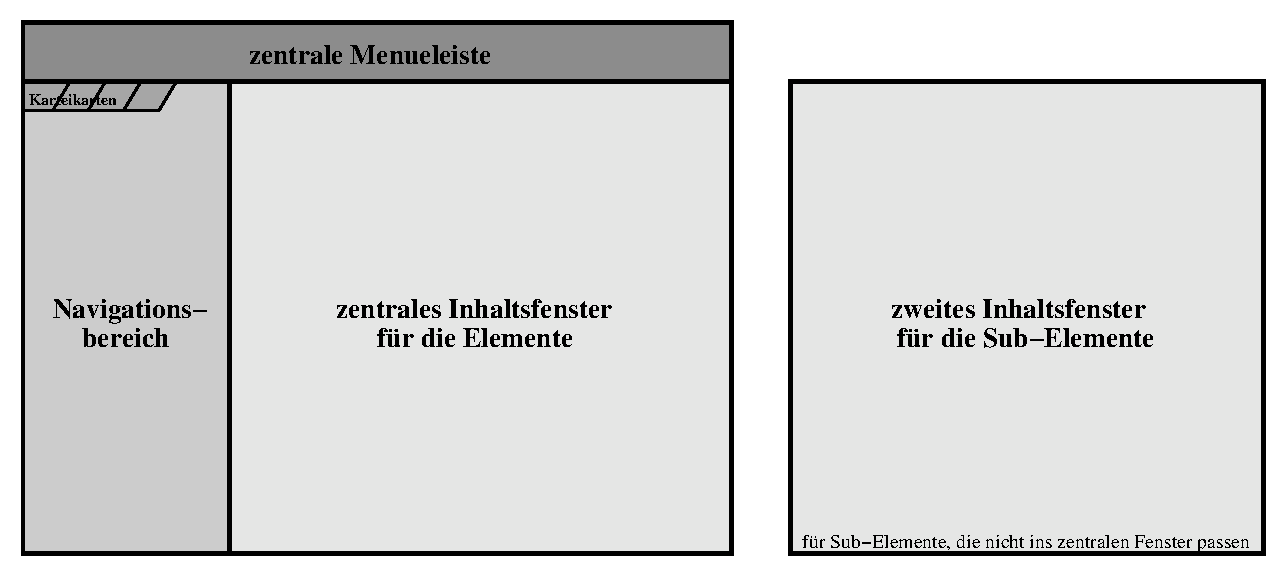
\epsfig{file=Skizzen/gesamtszenario_01.eps, height = 5cm}
\else
  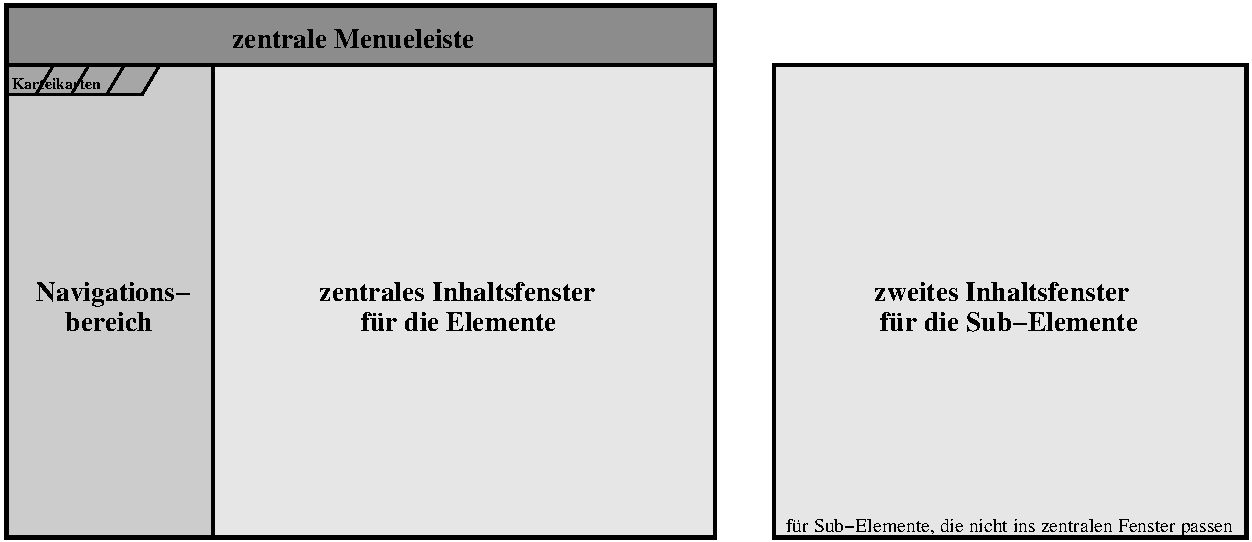
\includegraphics{Skizzen/gesamtszenario_01.pdf}
\fi
\caption{Layout der Hauptansicht im Lerntool}
\end{center}
\end{figure}                                   

Im folgenden werden diese Bereiche im Detail beschrieben.
                                  
%********************************************************************************

\clearpage

%********************************************************************************

\subsection{Zentrale Men"uleiste}

Die zentrale Men"uleiste besteht strukturell aus zwei Teilen:

\begin{list_sabina}
        \item \textbf{Graphischer Teil} f"ur Wechsel zwischen den
          verschiedenen Tools
        \item \textbf{Men"uteil} f"ur alle "ubrigen Funktionalit"aten\\
          (die i.a. weitere Unterstrukturen haben)
\end{list_sabina}                                                                                     

Die zentrale Men"uleiste ist (wie der Name sagt) ``zentral'' f"ur alle Tools der Mumie, \\
die Unterstrukturen des integrierten Pull-Down k"onnen jedoch verschieden
sein.\\
F"ur das Lerntool ergibt sich folgendes Bild:

\begin{figure}[h]
\begin{center}
\ifx\pdfoutput\undefined
  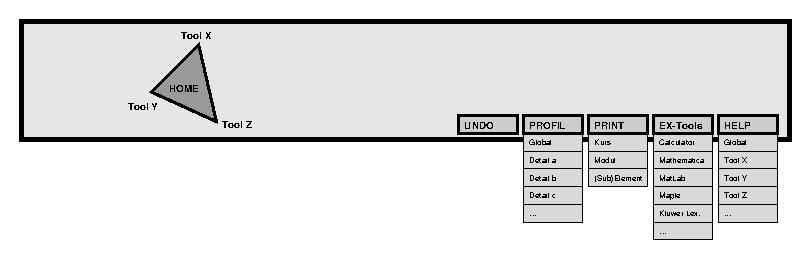
\epsfig{file=Skizzen/zent_menue.eps}
\else
  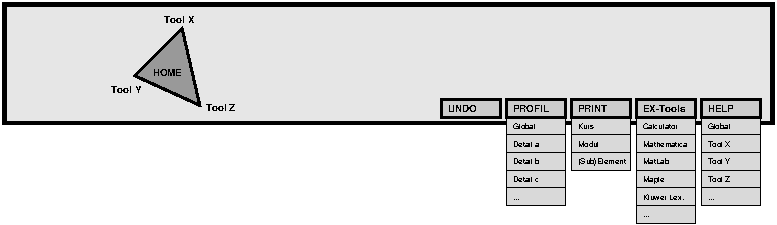
\includegraphics{Skizzen/zent_menue.pdf}
\fi
\caption{Layout der zentralen Men"uleiste}
\end{center}
\end{figure}                                   

Als ``Vorbild'' f"ur die Raumaufteilung zwischen Graphik- und Men"uteil und
auch f"ur die ungef"ahre Gr"o"se kann \verb?www.heute.t-online.de? gelten.
Der Graphische Teil sollte die Layout-Idee der Einstiegsseite aufgreifen.\\
Die detaillierte Entwicklung der Zentralen Men"uleiste ist damit der
Entwicklung des Gesamtlayouts zeitlich nachgeordnet (eventuell vereinfachte 
Dummyversion erstellen?).

%********************************************************************************

%\clearpage

%********************************************************************************

\subsection{Navigationsframe}

Details zum Navigationsframe werden derzeit in der separaten Spezifikation
``Navigationsframe'' (S.~Jeschke/E.~Zorn, November 2001) beschrieben.\\
Hier daher nur eine Zusammenfassung:

Der Navigationsbereich wird auf zwei verschiedene Weisen realisiert:

\begin{list_sabina}
        \item \textbf{Navigationsnetz}: Die Netzdarstellung erlaubt das orientierte
          Navigieren im gew"ahlten Kurs, stellt aber zus"atzlich weitere
          Elemente und alternative Wege dar, die jederzeit mit angew"ahlt
          werden k"onnen. \\
          Die Netzstruktur dient insbesondere der Vermittlung von
          mathematischen Zusammenh"angen: die logischen Abh"angigkeiten der
          Elemente werden durch eine Strichart (``logisches Netz''), 
          der gew"ahlte Kurs durch eine zweite Strichart (``Kurspfad'')
          dargestellt. Forward/Backward-Aktionen beziehen sich stets
          auf den Kurspfad.
        \item \textbf{lineare Navigation:} Die lineare Darstellung (Modell
          etwa wie ein U-Bahn-Plan f"ur eine einzige Linie) stellt nur die
          Elemente des Modules dar, die f"ur den gew"ahlten Kurs vorgesehen
          sind. Alternative Wege und/oder weitere vorhandene Elemente sind in
          dieser Darstellung unsichtbar.\\
          Die lineare Navigation dient insbesondere dem Ziel, dem 
          ``Lost-in-Cyberspace''-Effekt entgegenzuwirken.
\end{list_sabina}


Ausgangspunkt f"ur die Darstellung ist zun"achst das Navigationsnetz (hier
wird auf Alternativen erst aufmerksam gemacht, deren Existenz andernfalls
nicht sichtbar ist). Zwischen den beiden Navigationsformen kann zu jeden
Zeitpunkt geswitched werden (Karteikartensytem am oberen Rand des
Navigationsbereiches).
Zwischen den verschiedenen Ansichten (Navigationsnetz und Lineare
Navigation) wird durch ein Karteikartensystem hin- und hergeschaltet,
welches dar"uber hinaus weitere Karten verwaltet:

\begin{list_sabina}
        \item \textbf{1. Navigationsnetz}
        \item \textbf{2. Lineare Navigation}
        \item \textbf{3. Summary:}
        Zusammenfassung eines Modules \\
        (Stichwort: Vorschl"age nach V. En"s, to be specified)
        \item \textbf{4. Notes:}
        eigene Bemerkungen und Statusanzeigen, angelegt vom User \\
        (Stichwort: nach Linguistikprojekt, gesehen in K"oln, to be specified)
\end{list_sabina}

Die Karten werden durch Icons gekennzeichnet.\\
Aktivieren einer Karteikarte markiert deren Auswahl durch farbliche
"Anderung, highlighting etc.

Layouttechnisch muss das Auftreten von mindestens zwei weiteren
Karteikarten eingeplant werden (insbesondere auch im Hinblick auf die
"ubrigen Tools).

\begin{figure}[h]
\begin{center}
\ifx\pdfoutput\undefined
   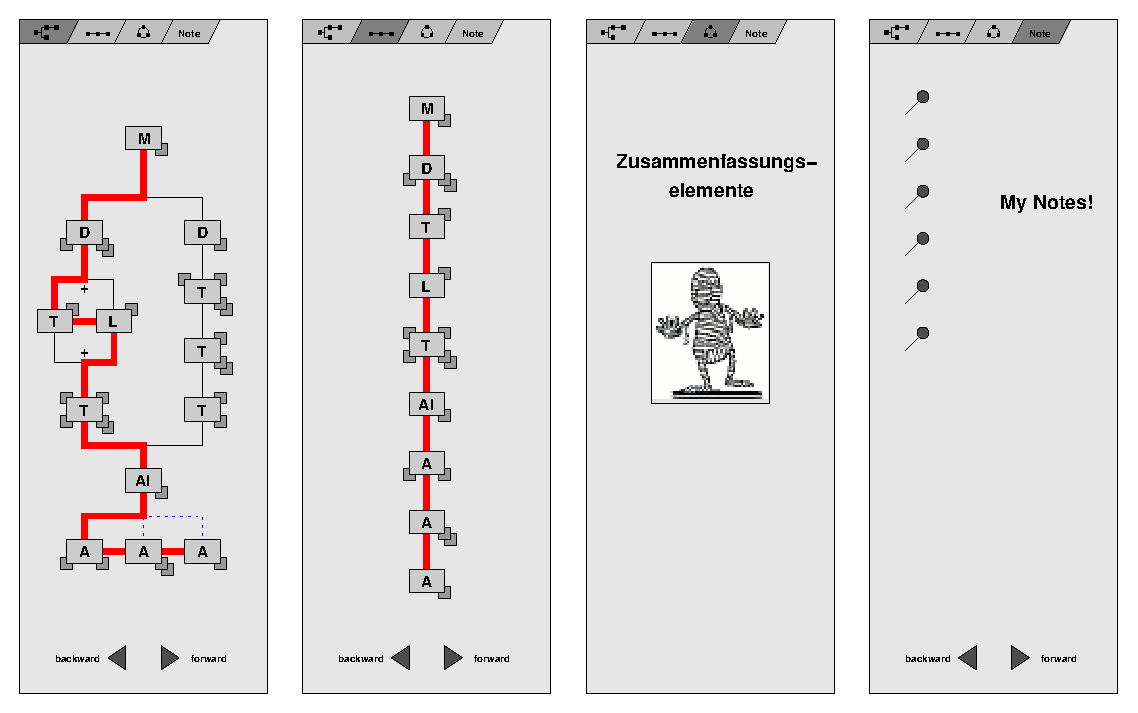
\epsfig{file=Skizzen/all_cards.eps, height=80mm} 
\else
  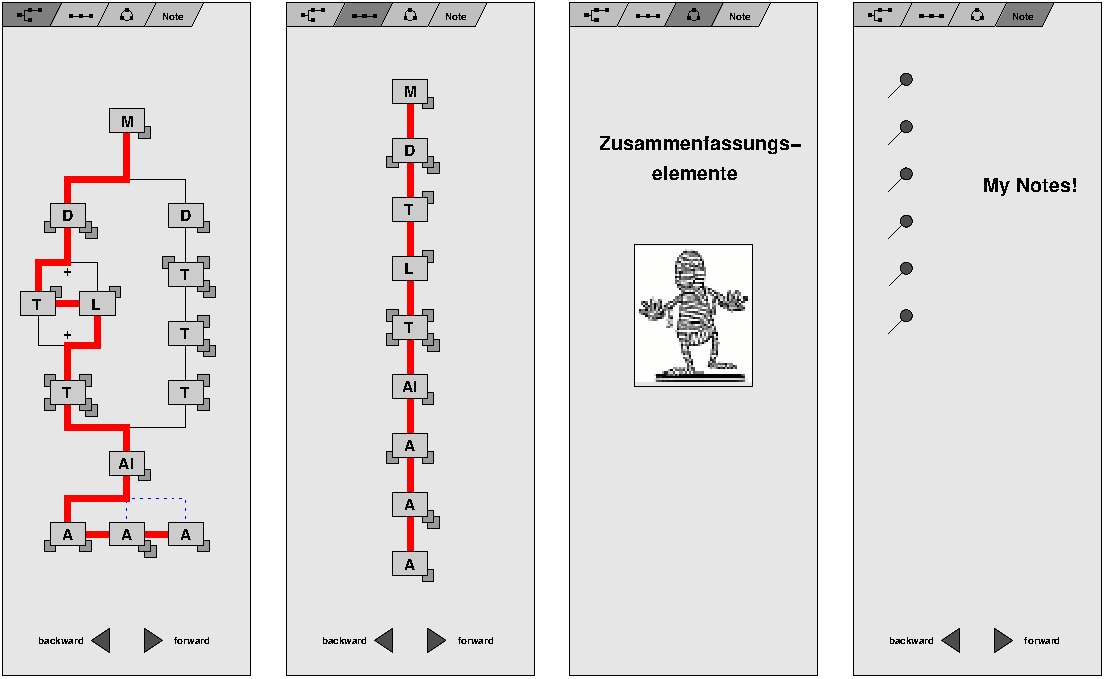
\includegraphics{Skizzen/all_cards.pdf}
\fi
\caption{Umschalten durch Karteikarten}
\end{center}
\end{figure}


%********************************************************************************

\clearpage

%********************************************************************************

\subsection{Zentrale Inhaltsfenster}


\subsubsection{Overview}


\subsubsection{Buttons}


\subsubsection{Integrierte}

